\begin{figure}[h]
\begin{center}
\includegraphics[width=0.7\linewidth]{images/transformer.png}
\end{center}
\caption{\textbf{Our model architecture.} }
\label{fig:model}
\end{figure}

\subsection{Expert Transformer}\label{sec:expert-transformer}

\paragraph{Patchify}
After being encoded into latent vectors of shape $T \times H \times W \times C$ by the 3D causal VAE, the video latents are patchified  along the spatial dimensions, resulting sequence $z_{\text{vision}}$ of length $T\cdot \frac{H}{p} \cdot \frac{W}{p}$. 
% VAE encodes the video into a latent vector of shape $T \times H \times W \times C$. Then we patchify the latent along the spatial dimensions, generating sequence $z_{vision}$ of length $T\cdot \frac{H}{p} \cdot \frac{W}{p}$. 
We do not patchify along the temporal dimension in order to enable joint training of images and videos.

\paragraph{3D-RoPE}
Rotary Position Embedding (RoPE)~\citep{su2024roformer} is a relative positional encoding that has been demonstrated to capture inter-token relationships effectively in LLMs, particularly excelling in modeling long sequences. To adapt to video data, we extend RoPE to 3D. 
Each latent in the video tensor can be represented by a 3D coordinate $(x, y, t)$.
We independently apply 1D-RoPE to each dimension of the coordinates, each occupies $3/8$, $3/8$, $2/8$ of the hidden states's channel. The resultsing encoding are then concatenate along the channel dimension to obtain the final 3D-RoPE encoding.

\paragraph{Expert Transformer Block}
We concatenate the embeddings of both text and video at the input stage to better align visual and semantic information. However, the feature spaces of these two modalities differ significantly, and their embeddings may even have different numerical scales. To better process them within the same sequence, we employ Expert Adaptive Layernorm to handle each modality independently.
As shown in Figure~\ref{fig:model}, following DiT~\citep{peebles2023scalable}, we use the timestep $t$ of the diffusion process as the input to the modulation module. 
Then, the Vision Expert Adaptive Layernorm and Text Expert Adaptive Layernorm independently apply this modulation mechanism to the vision hidden states and text hidden states respectively. This method promotes the alignment of feature spaces across two modalities while minimizing additional parameters.



\paragraph{3D Full Attention}
Previous works \citep{singer2022make, guo2023animatediff} often employ separated spatial and temporal attention to reduce computational complexity and facilitate fine-tuning from text-to-image models. However, as illustrated in Figure~\ref{fig:attention}, this separated attention approach requires extensive implicit transmission of visual information, significantly increasing the learning complexity and making it challenging to maintain the consistency of large-movement objects. Considering the great success of long-context training in LLMs and the efficiency of FlashAttention, we propose a 3D text-video hybrid attention mechanism. This mechanism not only achieves better results but can also be easily adapted to various parallel acceleration methods. 


\begin{wrapfigure}{r}{0.5\textwidth}
\centering
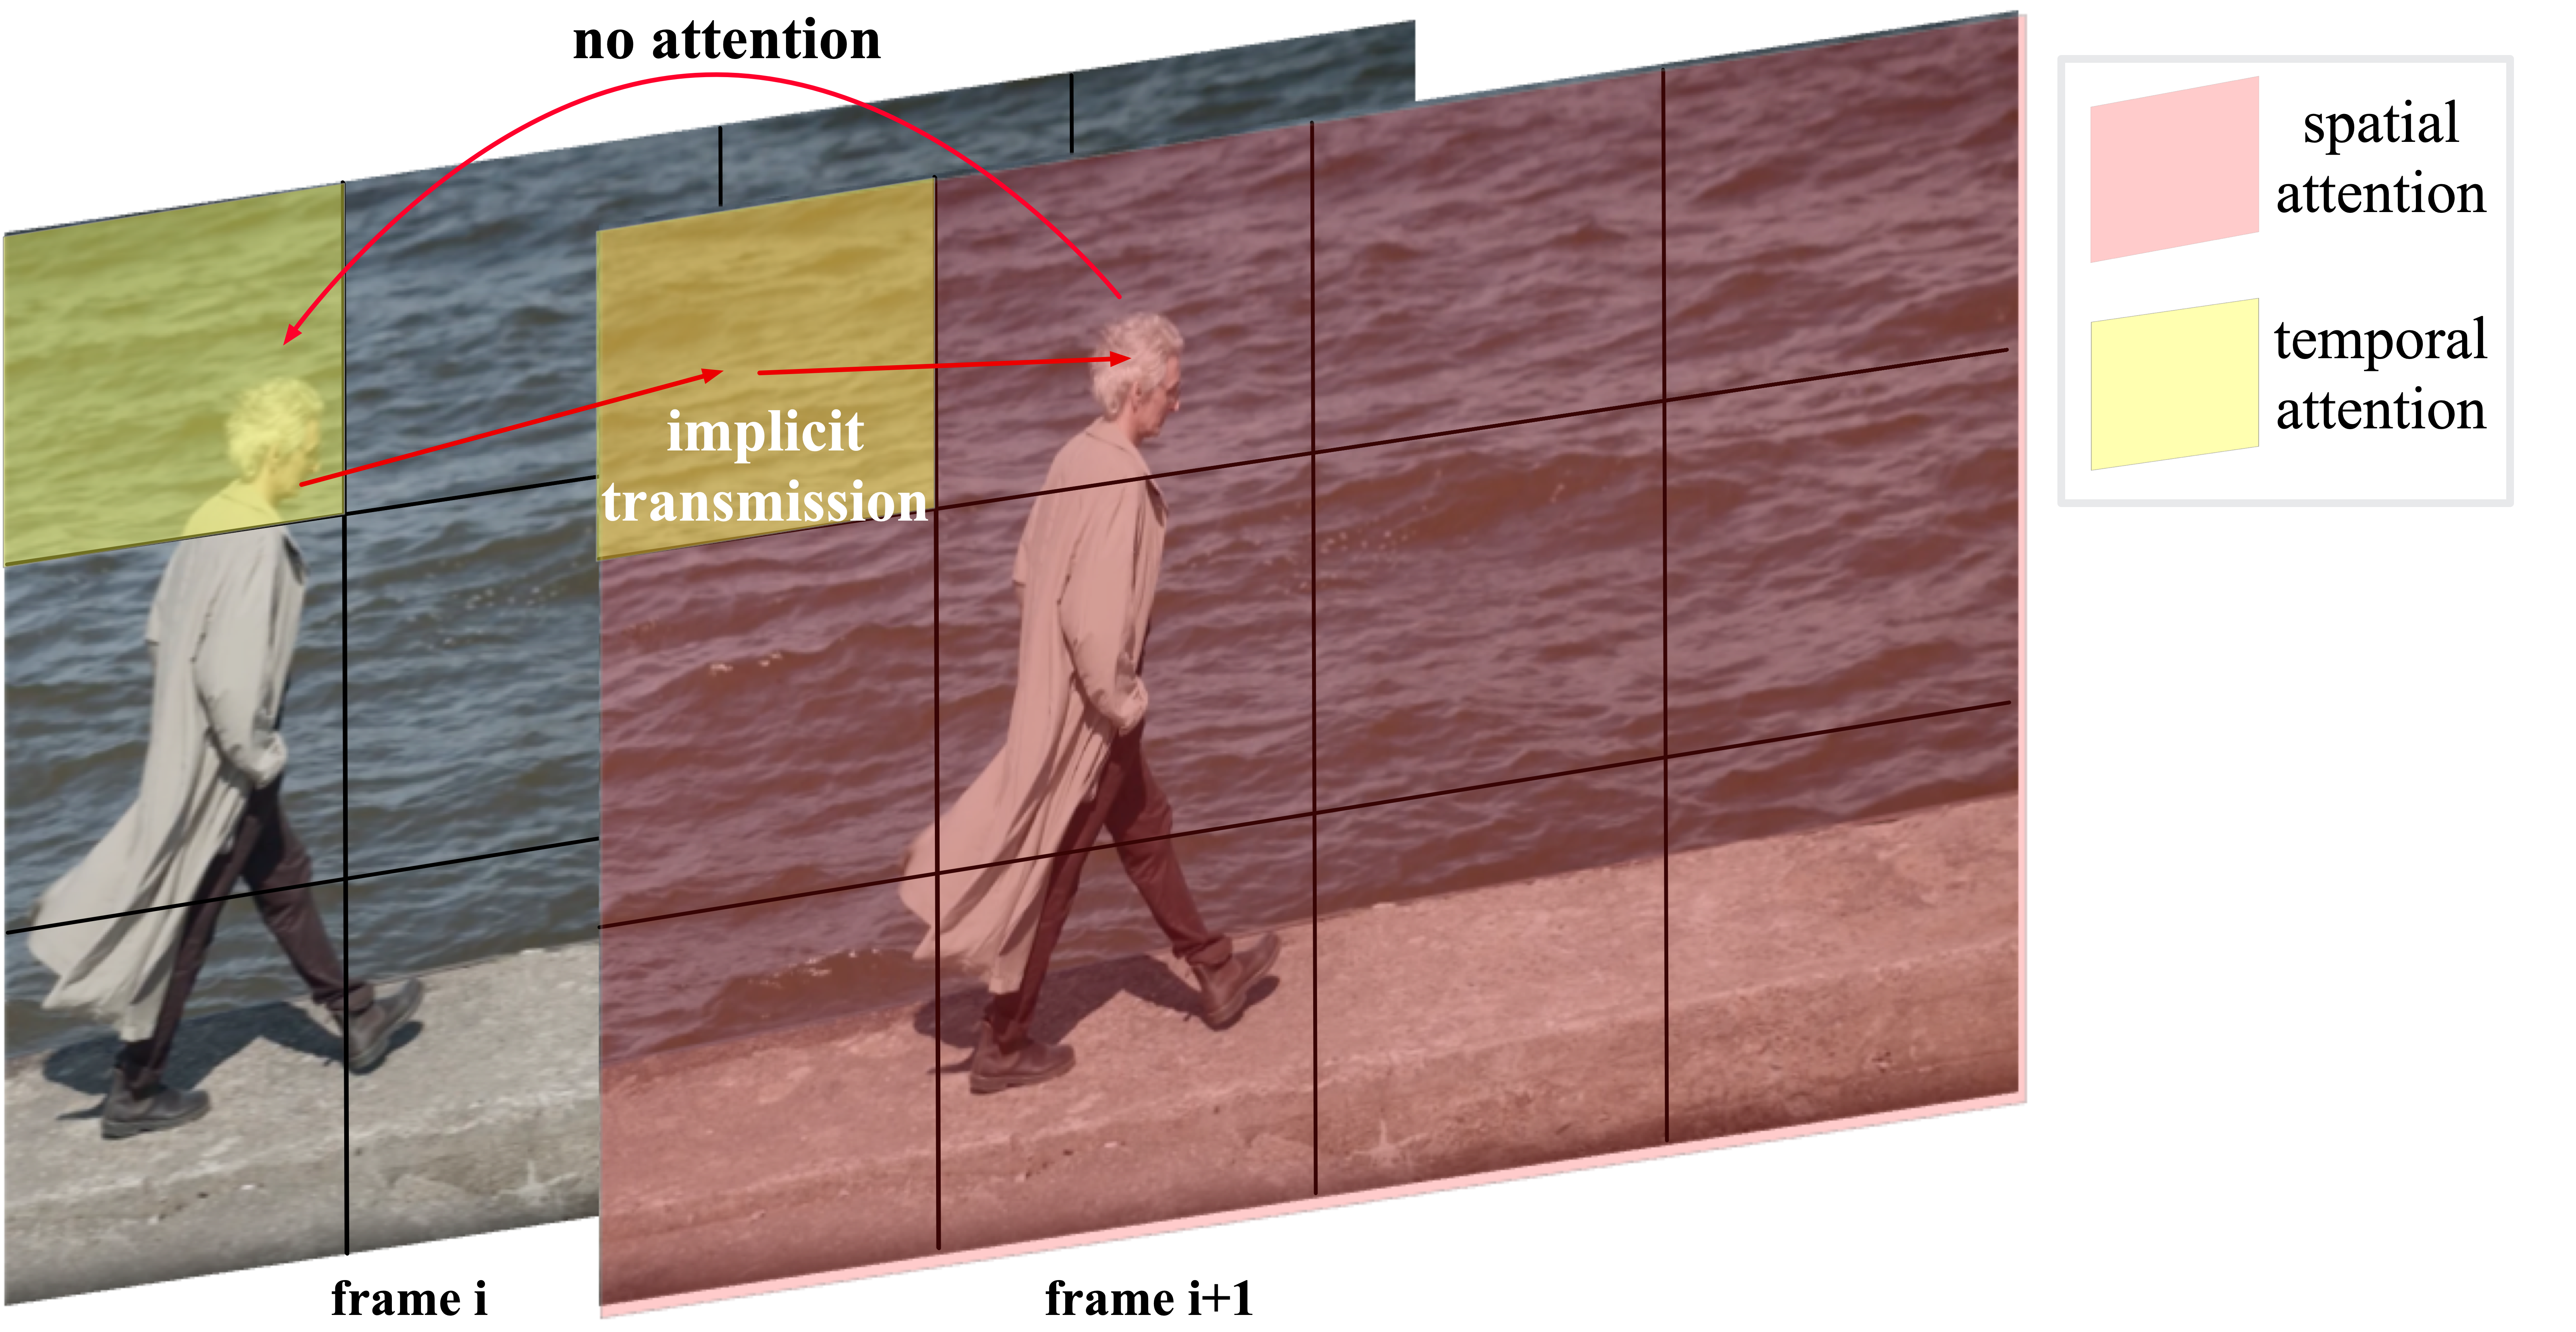
\includegraphics[width=\linewidth]{images/attention.png}
\caption{The separated spatial and temporal attention makes it challenging to  handle the large motion between adjacent frames. In the figure, the head of the person in frame $i+1$ cannot directly attend to the head in the frame $i$. Instead, visual information can only be implicitly transmitted through other background patches. This can lead to inconsistency issues in the generated videos.}
\label{fig:attention}
\vspace{-10mm}
\end{wrapfigure}



